\documentclass[12pt]{article}
\usepackage{amsmath}
\usepackage{amssymb}
\usepackage{geometry}
\usepackage{enumerate}
\usepackage{natbib}
\usepackage{float}%稳定图片位置
\usepackage{graphicx}%画图
\usepackage[english]{babel}
\usepackage{a4wide}
\usepackage{indentfirst}%缩进
\usepackage{enumerate}%加序号
\usepackage{multirow}%合并行
\title{\large UM-SJTU JOINT INSTITUTE\\PHYSICS LABTORATORY\\(VE216)\\\ \\\ \\\ \\\ \\\ \\\ \\\ \\\ \\\ \\\ \\\
LABTORATORY REPORT\\\ \\\ LAB 1\\\ LTI SYSTEMS \\\ \\\ \\\ \\\ \\\ }
\author{Name: Pan Chongdan\\ID: 516370910121\\Name Xiang Zhiyuan\\ID: 516370910126}
\date{Date: \today}

\begin{document}
\maketitle
\newpage
\section{Objectives}
\begin{itemize}
\item Become familiar with the laboratory equipment: power supply, signal generator, digital oscilloscope,
computer data acquisition system (Scope Connect).
\item Review basic concepts of linear time-invariant systems.
\item Illustrate several possible ways to determine the impulse response of a physical system from measured
data.
\item Use linearity, time-invariance and impulse response to compute the output of an LTI system when
the input is a step, a pulse, or a more complicated signal. 
\item Measure the output response of the series RC circuit for a variety of inputs, including a step, a
combination of a step and a ramp, and a sinusoid
\item Compare results to those computed as part of pre-lab assignment
\end{itemize}
\section{Theoretical Background}
An RC circuit is used so that the computations are easy and physically meaningful. The same procedures
can be applied to much more complicated systems.
\subsection{RC Circuit}
The RC circuit shown below is an example of a simple LTI system. Of course, there are many other LTI
systems that do not involve circuits at all.
\begin{figure}[H]
\centering
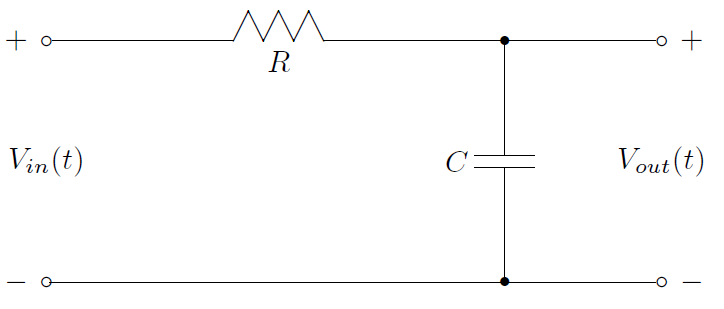
\includegraphics[scale=0.5]{p1.jpg}
\caption{RC Circuit}
\end{figure}
We will take the system input to be the voltage $V_{in}(t)$, while the system output is the voltage, $V_{out}(t)$,
dropped across the capacitor. Notice that these voltages, in general, will be functions of time,$t$.
\subsection{When is a Linear Circuit a Linear System?}
Using Kirchoffs current and voltage laws, one can easily derive a differential equation model of the RC-circuit
in Figure 1, namely
\begin{equation}
RC\frac{\mathbf{d}V_{out}(t)}{\mathbf{d}t}+V_{out}(t)=V_{in}(t)
\end{equation}
Appealing to basic knowledge of ODEs from a sophomore level math course, the total solution is seen to be
\begin{equation}
V_{out}(t)=V_0e^{-t/RC}+\int_0^t\frac{1}{RC}e^{-(t-\tau)/RC}V_{in}(\tau)d\tau,\tau>0
\end{equation}
where the initial condition at time zero is $V_{out}(0) = V_0$. It is very easy to verify that $V_{out}(t)$ is a linear
function $V_{in}(t)$ if, and only if, $V_{out}(0)=V_0=0$, that is, the initial voltage on the capacitor has to be zero.
This point is emphasized because you will have to assure this in the laboratory by either waiting for the
charge to decay on the capacitor or by shorting the capacitor with a wire.
\subsection{Impulse Response}
The impulse response, $h(t)$, of an LTI system is, by definition, the output response when the input of the
system is a delta function, $\delta(t)$. Of course, the delta function is a mathematical idealization. In practice,
$h(t)$ can be well approximated by the response of the system when the input is a pulse of very short duration
(compared with the response time of the system) and unit area, such as 
$p_{\bigtriangleup}=\frac{1}{\bigtriangleup}((u(t)-u(u-\bigtriangleup)))$ for $\bigtriangleup>0$ sufficiently small.
\par Note that in order to keep the area of the pulse equal to unity, the amplitude has to increase as the pulse
duration gets shorter. Often, this is a problem in a practical system as a large voltage pulse may fry an
amplifier, for example. One way to get around this is to use linearity and realize that if the input is scaled
by "$b$", then the output will be scaled by "$b$" as well. Consequently, if the measured response is divided by
"$b$", an approximation of the impulse response is obtained.
\subsection{Step Response}
For any LTI system the output can be expressed as
\begin{equation}
y(t)=x(t)*h(t)=\int_{-\infty}^\infty x(\tau)h(t-\tau)d\tau=\int_{-\infty}^\infty x(t-\tau)h(\tau)d\tau
\end{equation}
where $x(t)$ denotes the input and $*$ denotes the convolution operation. The output resulting when the input
is a unit step function, $x(t)=u(t)$, is called the unit step response. Simple manipulation leads to
\begin{equation}
y_{step}(t)=u(t)*h(t)=\int_{-\infty}^\infty h(\tau)u(t-\tau)d\tau=\int_{-\infty}^t h(\tau)u(t-\tau)d\tau+\int_t^\infty h(\tau)u(t-\tau)d\tau
\end{equation}
which, because the unit step function is equal to 1 for $t-\tau>0$ and equal to 0 for $t-\tau<0$ step response simplifies to
\begin{equation}
y_{step}(t)=\int_{-\infty}^th(\tau)d\tau
\end{equation}
By taking the derivative of $y_{step}(t)$ with respect to t, we obtain, by the fundamental theorem of calculus,
\begin{equation}
\frac{\mathbf{d}y_{step}(t)}{\mathbf{d}t}=\frac{\mathbf{d}}{\mathbf{d}t}\int_{-\infty}^th(\tau)d\tau=h(t)
\end{equation}
Thus the impulse response can be computed from the unit step response by calculating the derivative of the
step response with respect to time. This is a useful observation because it is sometimes easier to apply a
step input to a physical system than it is to apply (an approximation of) an impulse.
\par We now have two ways of determining the impulse response from data. A third way will be hinted at a
little later.
\section{Experimental Procedure}
\subsection{Step}
\begin{itemize}
\item Function generator: Utility $\to$ Output Setup $\to$ Load $\to$ High Z
\item Oscillator: Trigger Menu $\to$ 
$\begin{cases}
1.\text{Trigger Mode} \to \text{Basic}\\2.\text{Edge Trigger (Rising Edge)}\\\text{3.Trigger Settings} \to \text{DC Coupling} 
\end{cases}$
\item RC Circuit: $R=1K\Omega$, and $C=1\mu F$
\end{itemize}
\subsection{Part 1: Step Response} 
\begin{itemize}
\item Function generator:
\\Square Wave \qquad Vpp: 1V \qquad Frequency: 100Hz
\item Oscillator:
CH1: 200mV/div \qquad CH2: 200mV/div \qquad Time:2ms
\end{itemize}
\subsection{Part 2: Pulse Response}
\begin{itemize}
\item Function generator: Pulse frequency: 100Hz
\\1. Width: 1ms \qquad  A:100mV
\\2. Width: 0.5ms\qquad A:200mV
\end{itemize}
\subsection{Part 3: Ramp Response}
\begin{itemize}
\item Function generator:
\\Ramp \qquad Vpp:100mV \qquad frequency:100Hz
\end{itemize}
\subsection{Part 4: Sine Response}
\begin{itemize}
\item Function generator: 10 Vpp
\item Get the result of $V_{out}/V_{in}$, time shift and phase shift when the frequency is at 50, 500, 5000 respectively
\item Compare the results with ideal case
\end{itemize}
\section{Experimental Results}
\subsection{Part 1:Step Response}
\begin{figure}[H]
\centering
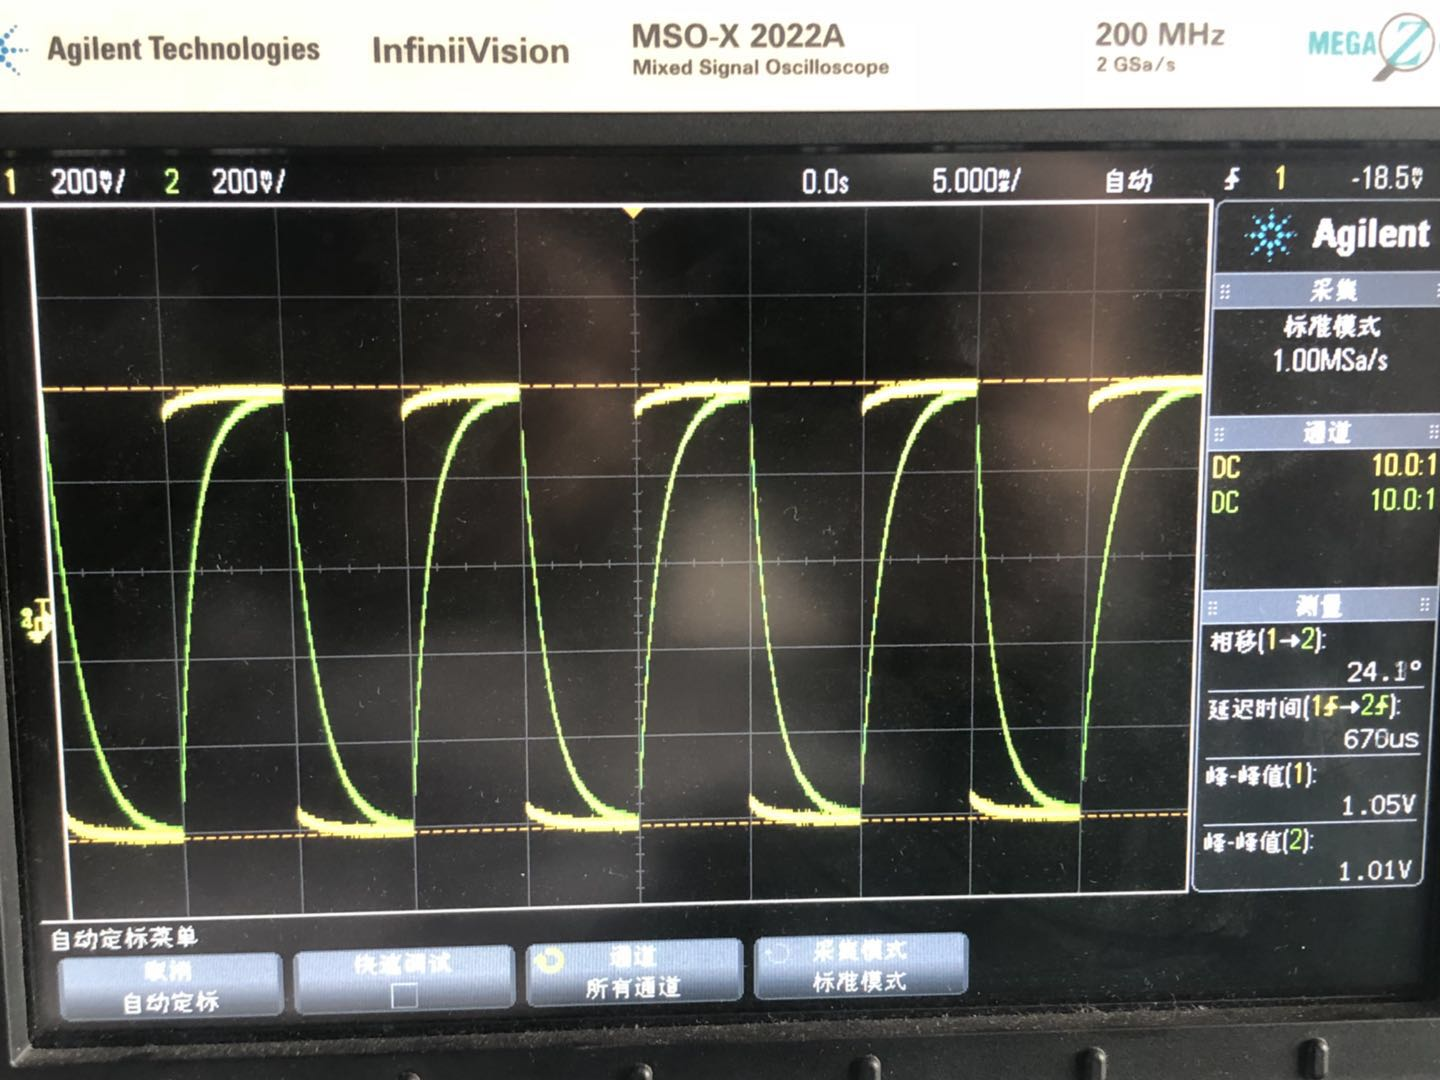
\includegraphics[scale=0.2]{p2.jpg}
\caption{Step Response}
\end{figure}
\subsection{Part 2:Pulse Response}
\begin{figure}[H]
\centering
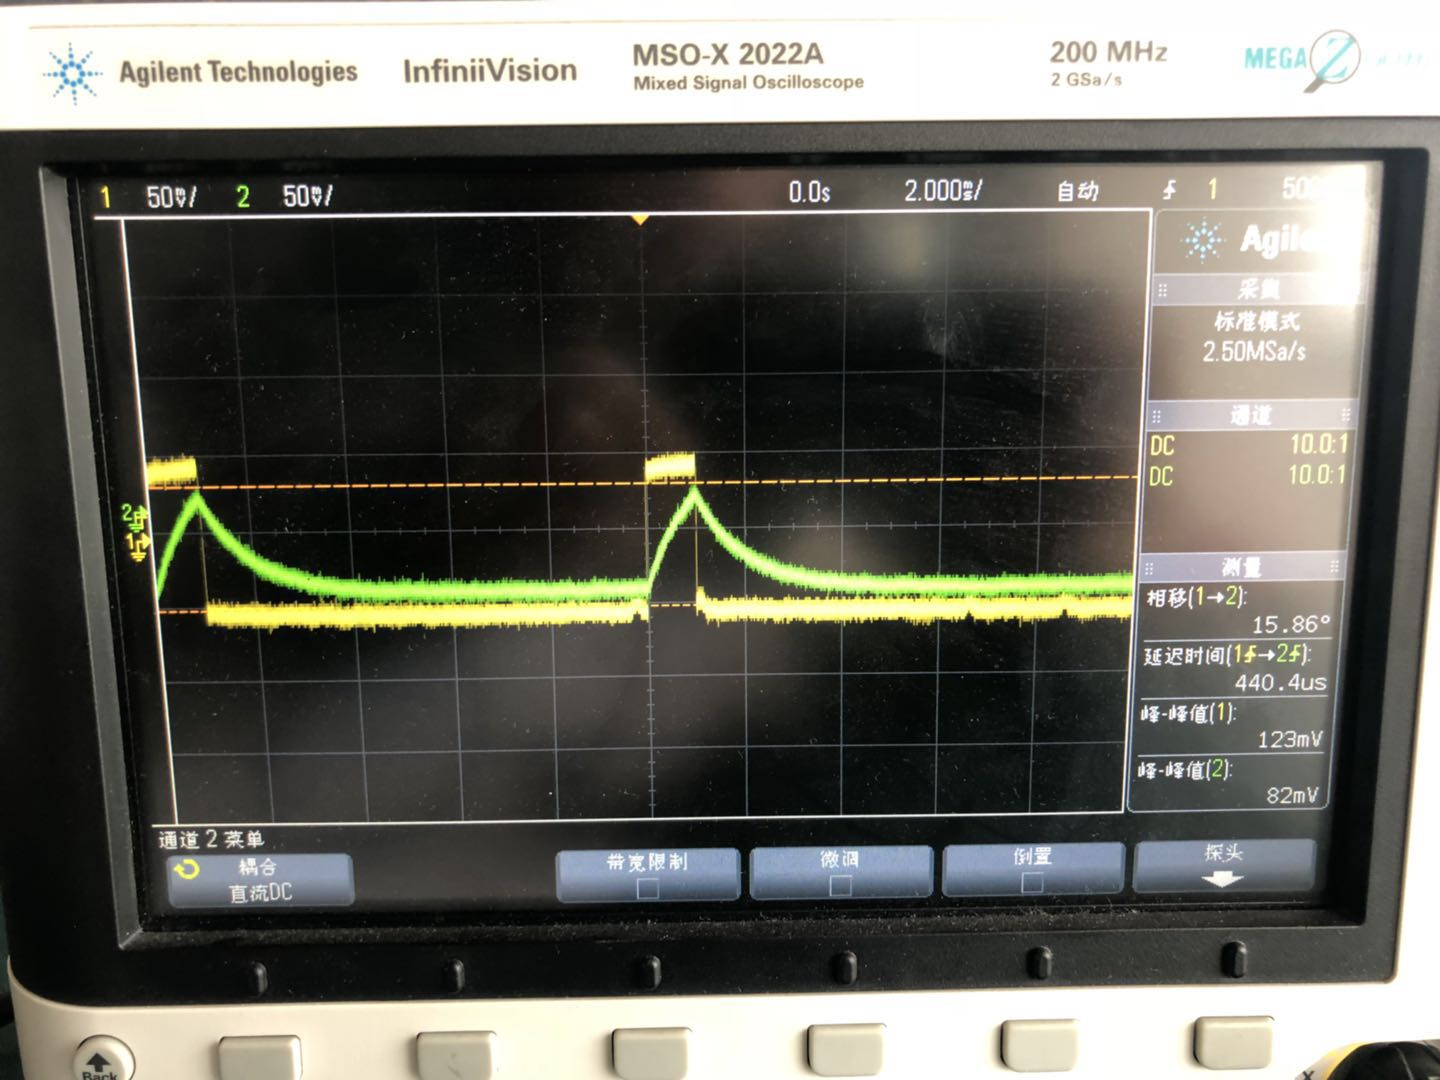
\includegraphics[scale=0.2]{p3.jpg}
\caption{Pulse Response 1}
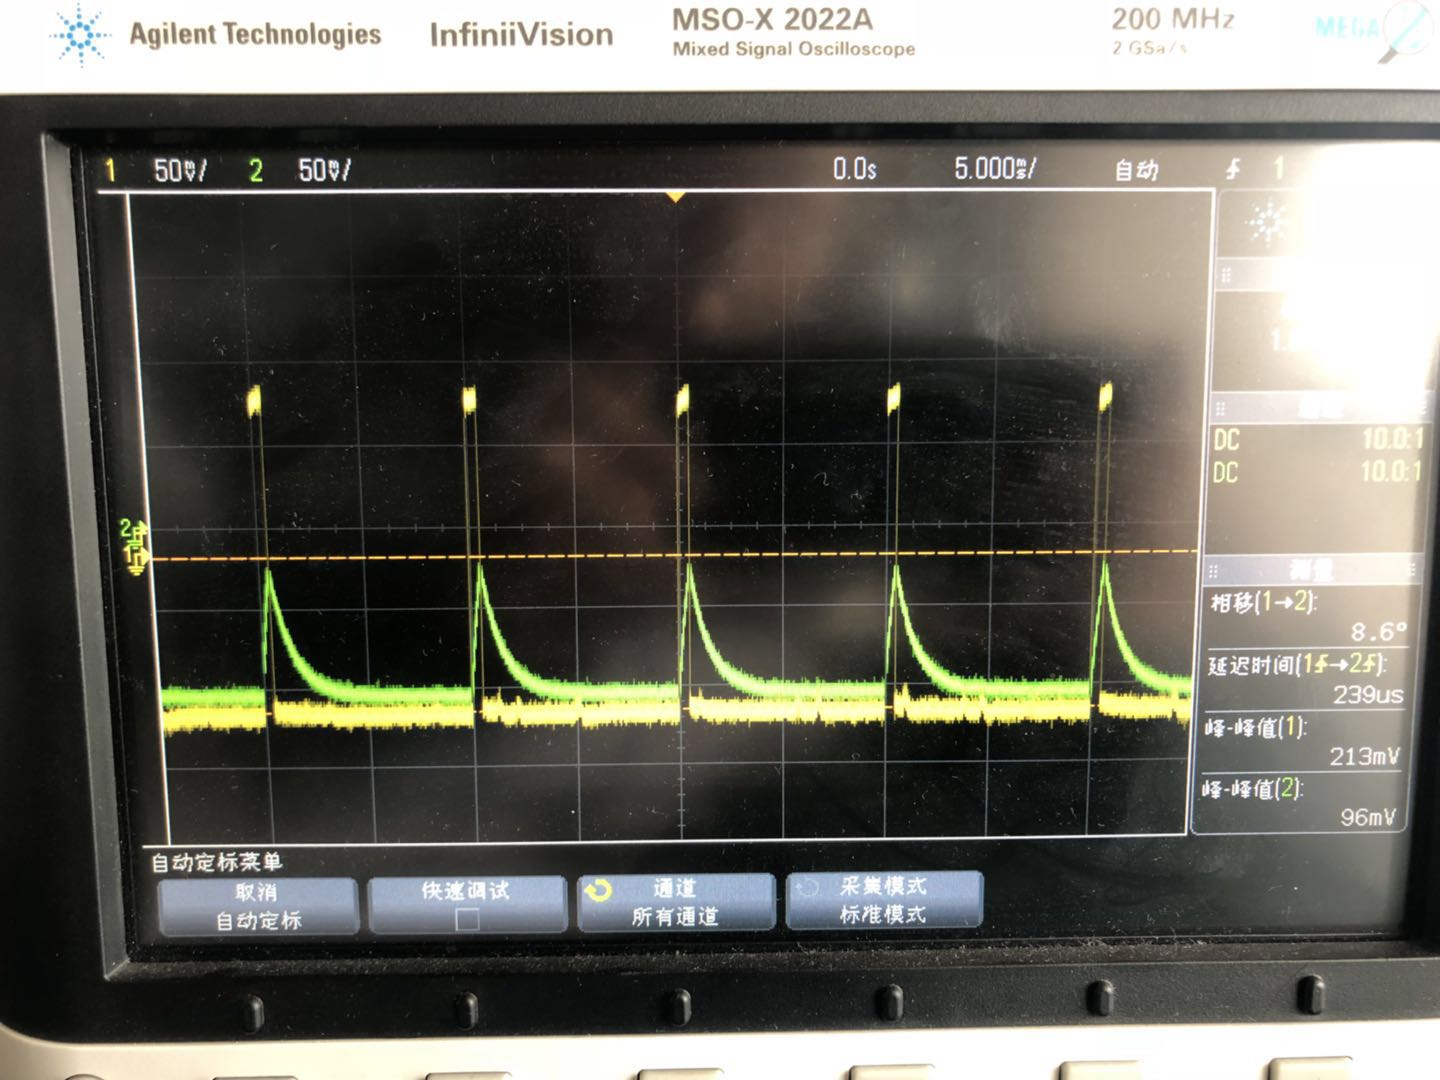
\includegraphics[scale=0.2]{p4.jpg}
\caption{Pulse Response 2}
\end{figure}
\subsection{Part 3:Ramp Response}
\begin{figure}[H]
\centering
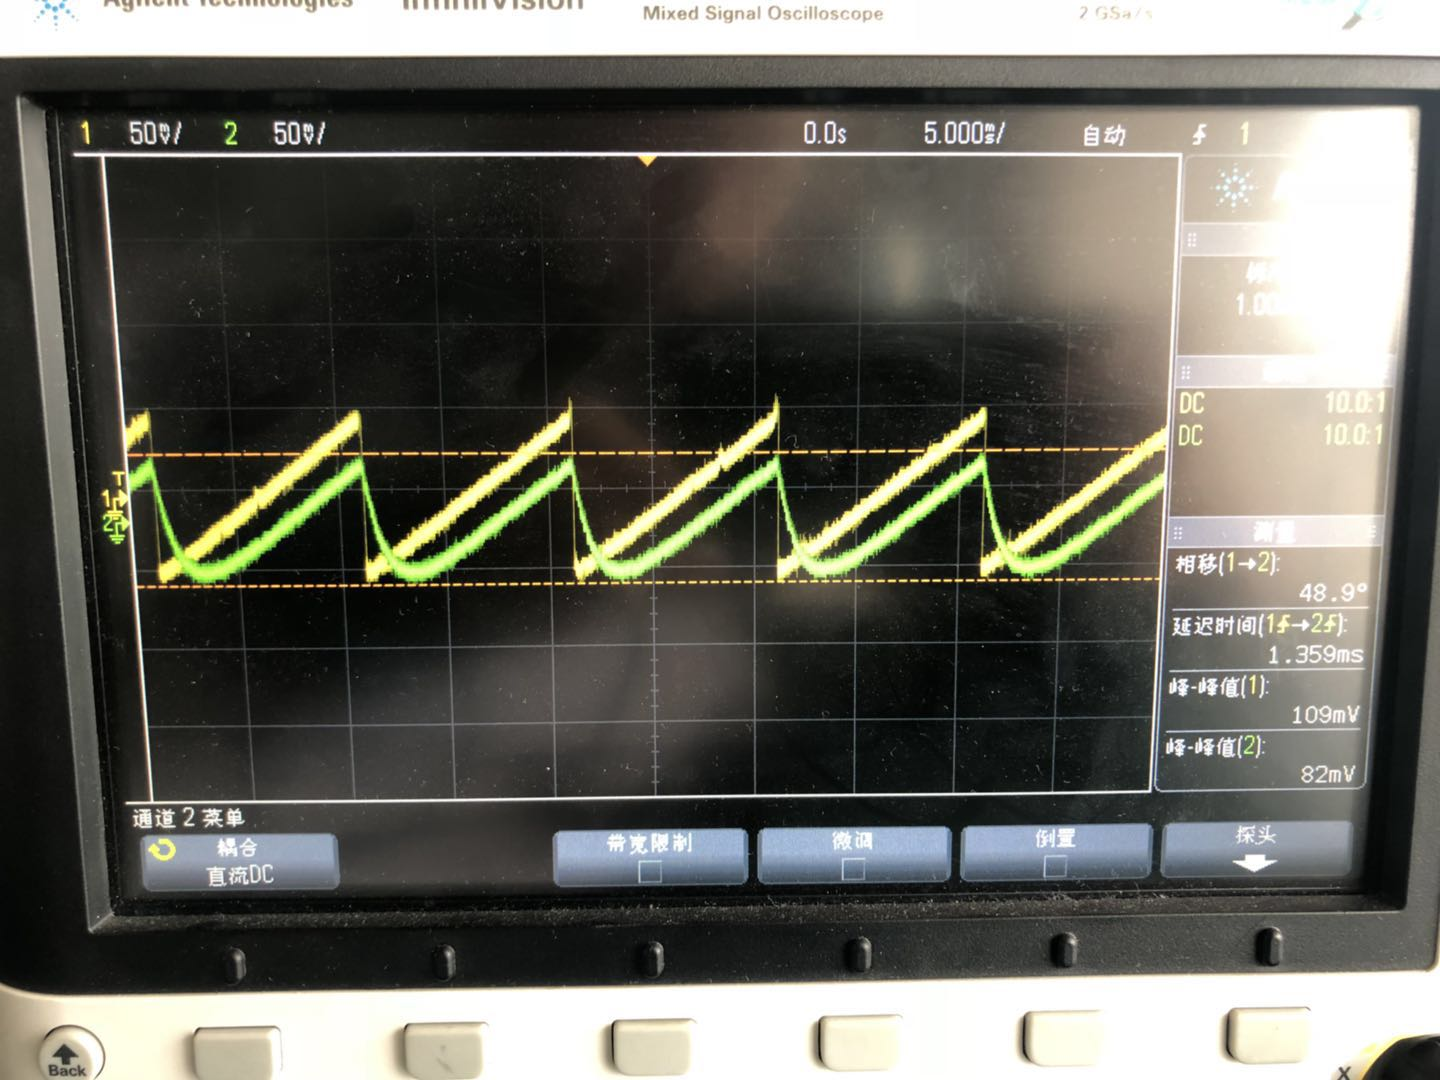
\includegraphics[scale=0.2]{p5.jpg}
\caption{Ramp Response}
\end{figure}
\subsection{Part 4:Sine Response}
\begin{table}[H]
\centering
\begin{tabular}{|c|c|c|c|}
\hline
Frequency (Hz) & Vout/Vin & Time Shift & Phase Shift \\ \hline
50             &0.9626          &1.02[ms]            &$-18.8^o$             \\ \hline
500            &0.3689          &410[$\mu$s]            & $-73^o$            \\ \hline
5k             &0.0359          &45[$\mu$s]            & $-82^o$            \\ \hline
\end{tabular}
\end{table}
\section{Error Analysis and Discussion}
\subsection{Error Analysis}
\subsubsection{Part 1:Step Response}
In our first part of the experiment, the square wave function can be formed by infinite step function, so we compare our figure with the step response, whose figure looks like this
\begin{figure}[H]
\centering
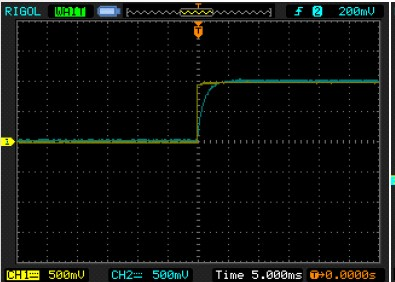
\includegraphics[scale=1]{p6.jpg}
\caption{Step Response}
\end{figure}
As we can see, this figures is quite similar to the one in experimental result, which means we got the right results in our first part.
\subsubsection{Part 2:Pulse Response}
In our second part, we dealt with the pulse train function, and compared our figure with the figure of pulse response
\begin{figure}[H]
\centering
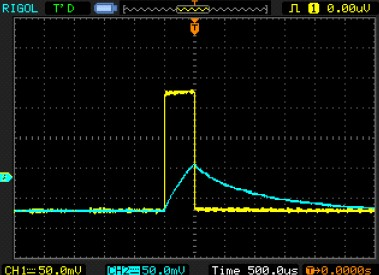
\includegraphics[scale=1]{p7.jpg}
\caption{Pulse Response}
\end{figure}
Also, its quite similar to the figure we got in experimental results, which means we got the right result in second part.
\subsubsection{Part 3:Ramp Response}
In the third part, compare our figure to the ramp response 
\begin{figure}[H]
\centering
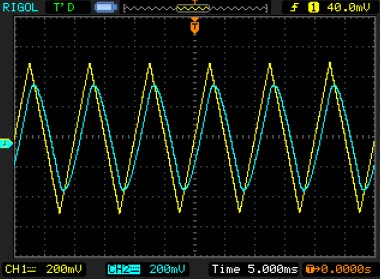
\includegraphics[scale=1]{p8.jpg}
\caption{Ramp Response}
\end{figure}
Obviously, our figure is quite same to the standard ramp response, so we succeed in getting the true results.
\subsubsection{Sine Response}
In part 4 we focused on the sine response, and figured out the values of $V_{out}/V_{in}$, Time Shift and Phase Shift at different Frequency(50Hz, 500Hz and 5kHz)
\begin{table}[H]
\centering
\begin{tabular}{|c|c|c|c|}
\hline
Frequency (Hz) & Vout/Vin & Time Shift & Phase Shift \\ \hline
50             &0.9626          &1.02[ms]            &$-18.8^o$             \\ \hline
500            &0.3689          &410[$\mu$s]            & $-73^o$            \\ \hline
5k             &0.0359          &45[$\mu$s]            & $-82^o$            \\ \hline
\end{tabular}
\caption{Experimental Results}
\end{table}
\qquad \\
\begin{table}[H]
\centering
\begin{tabular}{|c|c|c|c|}
\hline
Frequency (Hz) & Vout/Vin & Time Shift & Phase Shift \\ \hline
50             &0.9540          &0.9689[ms]            &$-17.4^o$             \\ \hline
500            &0.3033          &402[$\mu$s]            & $-72.3^o$            \\ \hline
5k             &0.0318          &49[$\mu$s]            & $-88.2^o$            \\ \hline
\end{tabular}
\caption{Theoretical Results Calculated in Prelab Exercise}
\end{table}
\qquad \\
\begin{table}[H]
\centering
\begin{tabular}{|c|c|c|c|}
\hline
Frequency (Hz) & Vout/Vin & Time Shift & Phase Shift \\ \hline
50             &0.0086          &0.0511[ms]            &$1.4^o$             \\ \hline
500            &0.0656          &8[$\mu$s]            & $0.7^o$            \\ \hline
5k             &0.0041          &4[$\mu$s]            & $6.2^o$            \\ \hline
\end{tabular}
\caption{Absolute Error}
\end{table}
\qquad \\
\begin{table}[H]
\centering
\begin{tabular}{|c|c|c|c|}
\hline
Frequency (Hz) & Vout/Vin & Time Shift & Phase Shift \\ \hline
50             &0.90\%          &5.27\%            &8.05\%             \\ \hline
500            &21.62\%          &1.99\%            &0.97\%            \\ \hline
5k             &1.29\%          &8.16\%          &7.03\%            \\ \hline
\end{tabular}
\caption{Relative Error}

\end{table}
As shown on the tables above, compare to the theoretical results we got before, they are quite close to each other, the relative error is below 8\%.
\subsection{Discussion of Error}
Though we did a good job and got the similar results comparing to the theoretical results, but there still are 4 errors in Part 4, we think there are 2 reasons.
\begin{enumerate}
\item First, is the unavoidable error, which is caused by the instruments we used. In the experiment, we were supposed to use the resistor with 1000$\Omega$, but actually, when we measured the resistor, the actual value is 985$\Omega$, and since in the ideal results, we assumed that $R$ is constant and equals to 1000$\Omega$, so obviously this will cause the errors, and it’s unavoidable since we can’t find a ideal resistor. Also, the connecting clamp might also have resistance, however, we ignore them in our ideal results.
\item Second, is the avoidable error, which is caused by ourselves. Though we called it the “avoidable error”, but actually it’s hard for us to avoid it, but we can try to decrease it. In the experiment, when we were reading the data from screen, actually the data is “shaking”, it was jumping up and down in a small range. And we just randomly chose one value in this range. This would cause some errors. To reduce the influence of this kind of errors, maybe next time we should choose the value which is exactly at the middle of the range, and repeat this experiment three or four times, choose the average value as the final answer.
\end{enumerate}
\section{Conclusion}
\subsection{Prelab}
By doing the prelab assignments, we take a review of the basic concepts of linear timeinvariant systems, like using the convolution to calculate the output signal. And also, we reviewed some knowledge about RC circuit we learned last year in Ve 215. And we got the ideal output when the input is a step, a pulse, or a more complicated siganl.
\subsection{During Lab}
We used and became familar with the laboratory equipments, like the power supply, signal generator and digital oscilloscope. By measuring the data and getting the figures by ourselves, we had a deeper understanding of the concepts in LTI system and RC circuit.
\subsection{After Lab}
we comparing the ideal results with the figures and data we got from the lab, and find they are quite similar to each other, which confirmed the concepts we learned before. Also, after we analyzing the errors, we got to know how to improve our steps next time.
All in all, this lab is quite successful, we got the results we want, we reviewed the previous knowledge and learned new knowledge at the same time.

\end{document}